%%%%%%%%%%%%%%%%%%%%%%%%%%%%%%%%%%%%%%%%
\section{Case Studies}
\label{sec:results}
%%%%%%%%%%%%%%%%%%%%%%%%%%%%%%%%%%%%%%%%

The pytokio package and its accompanying services described in Sections \ref{sec:architecture} and \ref{sec:apps} provide the interfaces and infrastructure necessary to explore I/O performance in a holistic manner.
To demonstrate this, we present several case studies where pytokio has been applied to solve specific operational problems or gain new insight into storage system behavior.
In all cases, file system traffic data archived using the pytokio archival service is combined with data from other sources such as Darshan to identify and confirm behavior that would otherwise be ambiguous from a single component-level monitoring tool.

\subsection{Performance analysis of individual jobs} \label{sec:results/users}

\begin{figure}
    \centering
	\subfloat[Correlation between I/O performance and Lustre OST]{%
    	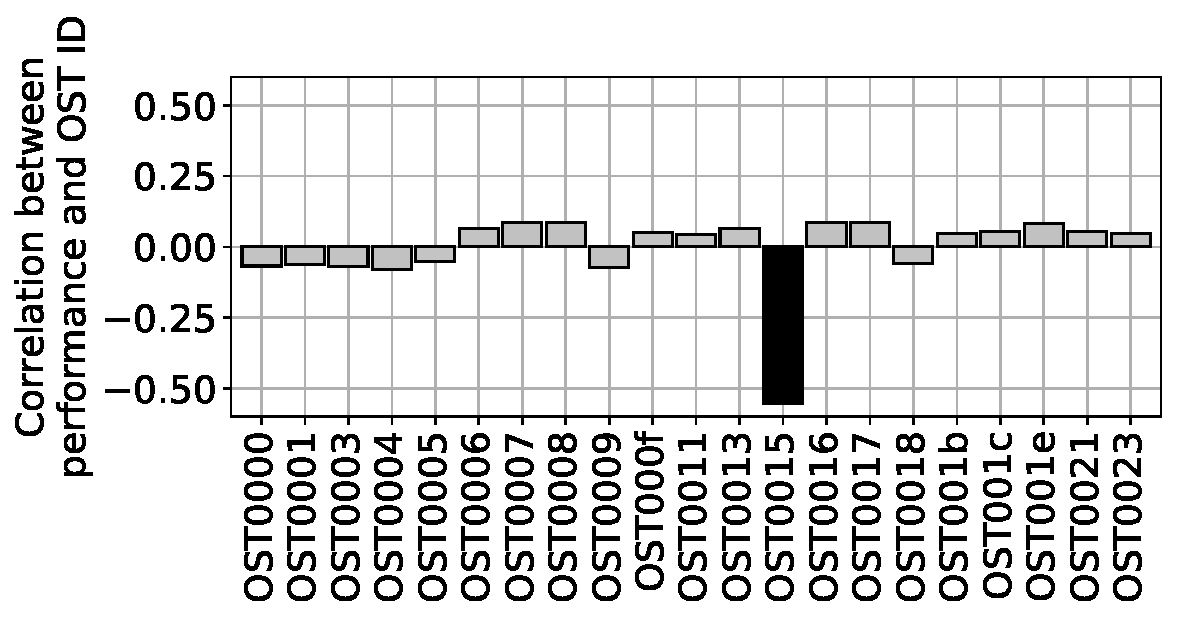
\includegraphics[width=0.9\linewidth]{darshan_bad_ost}
	    \label{fig:straggling-ost/correlation}
    }
    \\
    \subfloat[Per-OST performance over time]{%
    	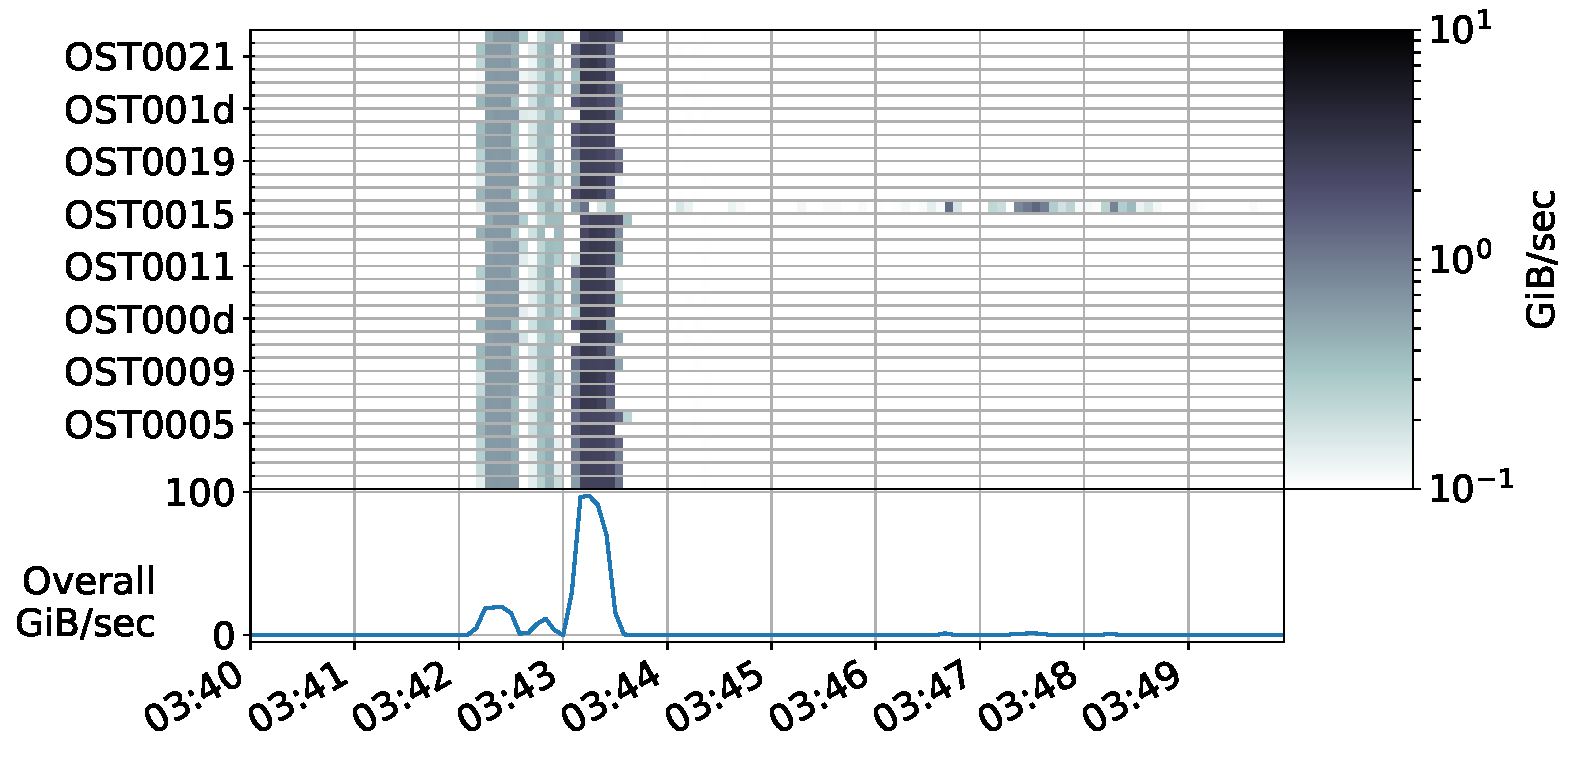
\includegraphics[width=0.9\linewidth]{heatmap_straggler}
    	\label{fig:straggling-ost/heatmap}
    }

    \caption{%
    (a) Correlation between per-file application I/O performance and the OSTs to which each file was mapped (from Darshan); shading indicates statistical significance, with darker bars being more significant.
    (b) Per-OST I/O performance measured over the same time that the job in (a) was running (from LMT).
    In both (a) and (b), OST0015 is identified as showing abnormally poor performance.
    }
    \label{fig:straggling-ost}
    \vspace{-.2in}
\end{figure}

Answering the question of why I/O was slow for a user's job was one of the principal motivators behind developing pytokio, and the UMAMI approach described in Section \ref{sec:apps/analysis} goes a long way towards answering this question.
In the absence of a series of jobs with similar I/O patterns from which an UMAMI diagram can be assembled, though, the \texttt{summarize\_job} tool can still provide useful metrics such as the degree to which the user's job experienced I/O contention with others (its coverage factor~\cite{Lockwood2017}).

However, there are some causes of poor I/O performance that are not well resolved by spatially reduced data as is provided by \texttt{summarize\_job}.
For example, a single slow Lustre OST can dramatically impact overall I/O performance~\cite{Byna2013}, but detecting this condition requires examining the performance of each OST individually.
Because the specific malady of a straggling OST is sufficiently common in highly parallel Lustre systems, pytokio includes a \texttt{darshan\_bad\_ost} analysis tool that attempts to statistically identify slow OSTs using the per-file performance and OST mappings contained in Darshan logs.

This tool first estimates per-file I/O bandwidths by dividing the total bytes read/written to each file by the time the application spent performing I/O to that file.
It then uses data from Darshan's Lustre module~\cite{Snyder2016modular} to map these performance estimates to the OSTs over which each file was striped.
With the list of OSTs and performance measurements corresponding to each OST, the Pearson correlation coefficient is then calculated between performance and each individual OST.

Figure \ref{fig:straggling-ost/correlation} shows the result this correlation analysis for a slow-running job that performed file-per-process I/O to files with a stripe width of 1 on NERSC Edison's ``scratch3'' Lustre file system.
For almost all OSTs, the correlation between performance and OST ID wavers around zero, indicating minimal correlation.
However, OST0015 stands out in stark contrast; it correlates strongly and negatively with performance. 
This inverse relationship between file I/O performance and files existing on this OST suggests that this OST is in an unhealthy state and is not delivering the same level of performance as its peers.

To confirm that OST0015 is indeed behaving abnormally relative to its peers, spatially resolved bandwidth measurements from the LMT connector can be retrieved using the pytokio LMT tool and rendered using a heatmap visualization notebook provided with pytokio.
The result of this temporally and spatially resolved OST performance is shown in Figure \ref{fig:straggling-ost/heatmap}.
Whereas almost all OSTs during this job's write phase were able to complete their I/O between 3:43 AM and 3:44 AM, OST0015 shows a long tail of performance, with relatively little I/O activity between 3:43 AM and 3:44 AM but I/O activity still occurring as late as 3:48 AM.
Using both statistical analysis of Darshan data and a visualization of high-resolution LMT data, the poor performance of this job can be confidently attributed to a poorly performing OST.

While this method is a useful user-facing tool for performance analysis, it can also be a valuable tool for systems engineers.
A number of HPC facilities perform automated, daily I/O benchmarks to establish baseline levels of performance variation\cite{Lockwood2017,Simakov2015}.
Automatically inspecting the Darshan logs from these performance probes using  \texttt{darshan\_bad\_ost} enables the detection of more complex, fail-slow scenarios caused by individual component degradations~\cite{Gunawi2018}.
Automatically running \texttt{darshan\_bad\_ost} with appropriate correlation and significance thresholds allows HPC operators to be alerted whenever a Darshan log is generated that implicates a subset of OSTs as causing overall performance degradation.

%%%%%%%%%%%%%%%%%%%%%%%%%%%%%%%%%%%%%%%%
\subsection{User engagement for burst buffers}
\label{sec:results/bb}
%%%%%%%%%%%%%%%%%%%%%%%%%%%%%%%%%%%%%%%%

\begin{figure}
    \centering
    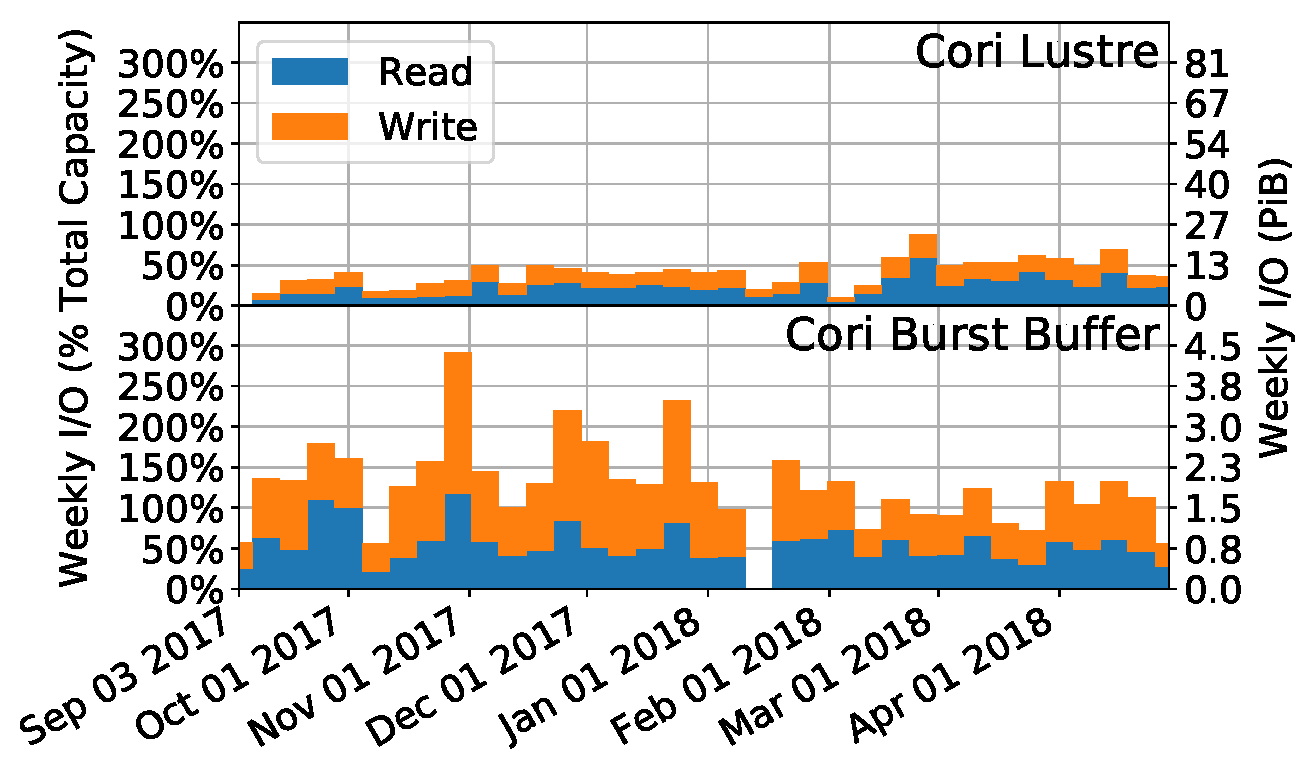
\includegraphics[width=1.0\linewidth]{cori-weekly-traffic}
    \caption{%
    Total I/O traffic read and written to Cori's Lustre file system (top, obtained from LMT) and DataWarp burst buffer (bottom, obtained from SMART data) per week.
    Left axis expresses I/O volumes normalized to the total capacity of each storage system; right axis shows the absolute I/O volumes in PiB ($2^{50}$ bytes).
    Overall read/write ratios are 0.568 (Lustre) and 0.429 (Burst Buffer).
    }
    \label{fig:cori-weekly-traffic}
    \vspace{-.2in}
\end{figure}

DataWarp-based burst buffers enable users to dynamically provision high-performance flash storage in the form of scratch instances that provide private, ephemeral parallel file systems~\cite{Henseler2016}.
Although this enables much higher, more reliable performance than a globally shared Lustre file system, users must consciously incorporate DataWarp into their application workflows to realize these benefits.
The ``opt-in'' nature of DataWarp, NERSC's steady stream of new users, and a general lack of awareness of I/O issues results in a number of NERSC users continue to rely exclusively on Cori's Lustre file system for their I/O-intensive workloads despite the potential benefits of Cori's burst buffer.

To determine how well balanced the utilization of the Lustre file system and DataWarp burst buffer are, NERSC uses a pytokio-based service that provides automated reporting on the total I/O traffic reported by both storage systems.
Figure \ref{fig:cori-weekly-traffic} shows the amount of bytes read from and written to both Cori's Lustre file system and burst buffer on a weekly basis.
The burst buffer sees traffic equivalent to 120\% of its total capacity moved every week on average, while Cori's Lustre file system averages 39\%.
Because Cori's Lustre is ${> 17 \times}$ more capacious than its burst buffer, though, these I/O volumes reflect a significant disparity--the burst buffer sees 1.85 PiB/week of traffic, while the Lustre file system sees 10.6 PiB/week.
Furthermore, Cori's Lustre capacity fills at a rate of $\approx 10\%$ of its weekly write volume, indicating that a significant amount of this Lustre traffic is for temporary data that is not retained.

These data confirm that, despite the availability of Cori's burst buffer, Cori's Lustre file system still experiences a significant amount of scratch-like I/O traffic.
In addition, the write volumes for the burst buffer in Figure \ref{fig:cori-weekly-traffic} reflect an average of 0.117 drive writes per week, while the SSDs in Cori's burst buffer are rated for 70 drive writes per week.
Thus, we can conclude that Cori's Lustre file system still has a significant amount of scratch-like I/O it can shed to the burst buffer, 
and the burst buffer has more than enough endurance to sustain such an increase in its workload.

\begin{figure}
    \centering
    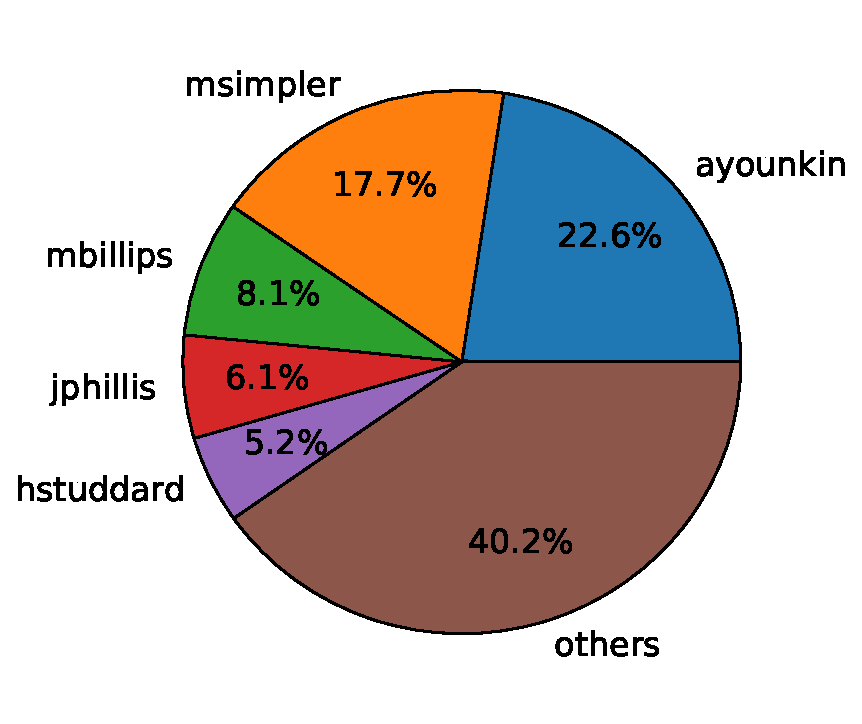
\includegraphics[width=0.75\linewidth]{darshan-month-pie}
    \vspace{-.2in}
    \caption{%
    Top five I/O users on the Cori Lustre file system during April 2018 as measured by Darshan.
    Data only reflects I/O performed by MPI applications that produced valid Darshan logs.
    User names shown are pseudonyms.
    }
    \label{fig:darshan-month-pie}
    \vspace{-.2in}
\end{figure}

To identify workloads that may be good candidates for migration to Cori's burst buffer, NERSC continuously monitors the application I/O load data targeting Lustre.
A pytokio-based service scans and indexes the Darshan logs generated by user jobs on Cori on a daily basis at NERSC to simplify the process of identifying jobs that perform significant I/O to a specific file system.
pytokio also includes the \texttt{darshan\_scoreboard} command-line tool that enables simple querying of these Darshan log indices to determine which applications and users are generating the highest I/O traffic.
Combining these tools results in a daily, weekly, or monthly ``scoreboard'' that identifies the individuals producing the most significant I/O to each storage system.
An example of such a scoreboard is shown in Figure \ref{fig:darshan-month-pie}, which reveals that almost 60\% of the I/O traffic captured by Darshan is generated by five users.

Simultaneously, NERSC continuously monitors the file system traffic data targeting Cori's burst buffer to monitor its utilization and wear rate.
With these two pytokio-derived services, NERSC staff receive regular automated reports that indicate (1) which users are responsible for the largest fraction of I/O traffic to Lustre, and (2) when the burst buffer is not being heavily utilized.
With this information, staff are able to engage with specific users about migrating their workload to use the burst buffer, effecting significant impact on both improving performance for major I/O workloads and reducing the load on the Lustre file system for other users.

%%%%%%%%%%%%%%%%%%%%%%%%%%%%%%%%%%%%%%%%
\subsection{Identifying major factors affecting performance} \label{sec:results/fs-behavior}
%%%%%%%%%%%%%%%%%%%%%%%%%%%%%%%%%%%%%%%%

\begin{figure*}
    \centering
    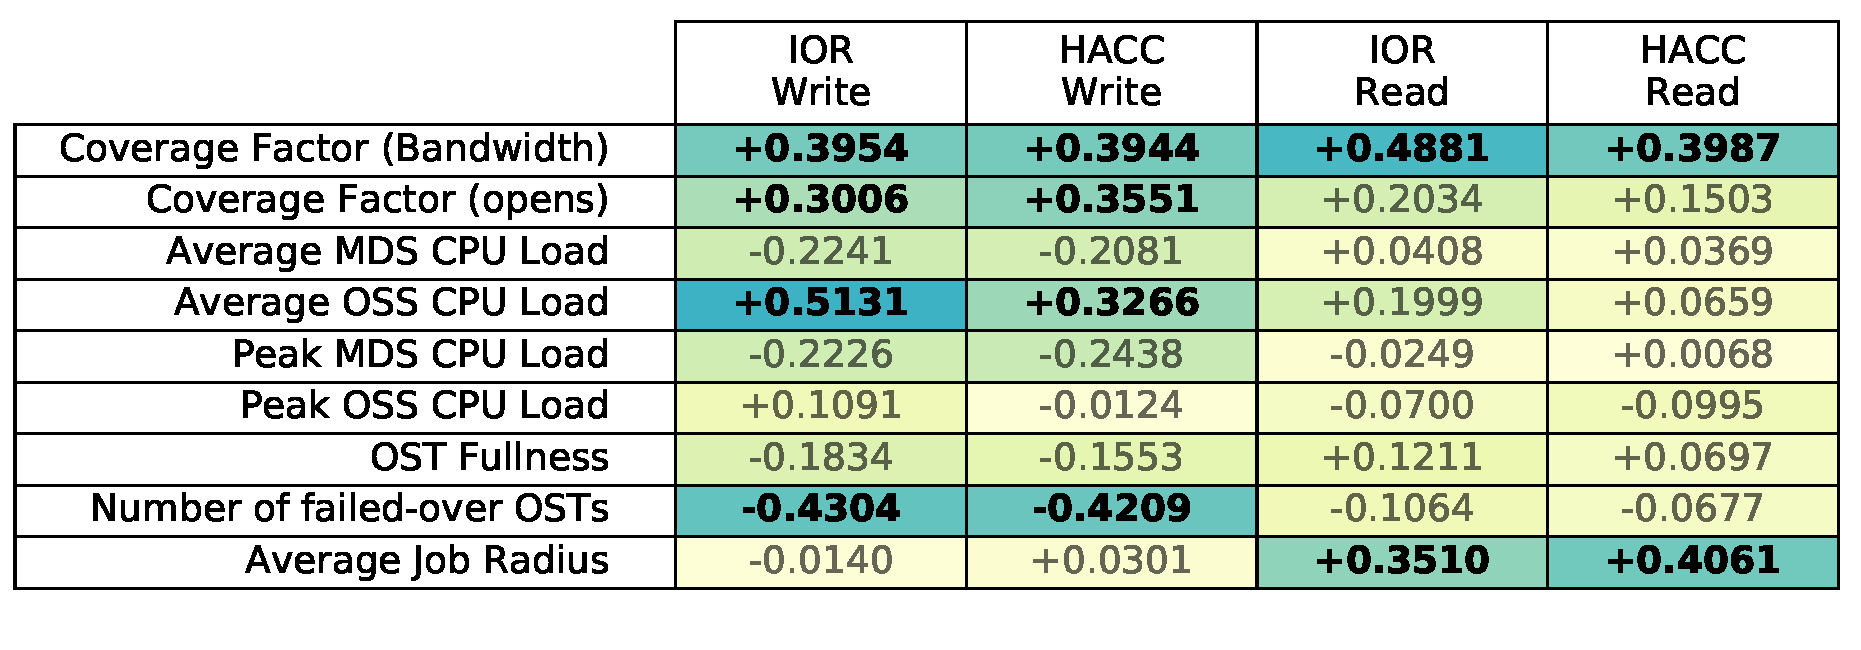
\includegraphics[width=0.75\linewidth]{correlation_table_fpp_writes}
    \caption{Pearson correlation between application I/O performance and other metrics collected by pytokio on NERSC's Cori system.
    Each value is shaded according to the magnitude of the positive or negative correlation, and values printed in bold are statistically significant (p-value $ < 10^{-5}$) whereas other values are not.
    The IOR benchmarks used 4,096 processes to read and write 16 TiB of data using 4 MiB transfers.
    The HACC benchmarks used 4,096 processes to read and write 8 TiB of data using $\approx$ 128 MiB transfers.
    Data reflects daily benchmark results obtained between February 14, 2017 and February 15, 2018.
    }
    \label{fig:correlation-table}
    \vspace{-.2in}
\end{figure*}

Daily I/O benchmarks can be used to develop a quantitative understanding of how different components of the I/O subsystem affect I/O performance.
Applying \texttt{summarize\_job} to collect all available telemetry associated with daily benchmarks provides a series of performance snapshots \emph{and} the factors that contributed to that performance.
By applying simple correlation analysis--calculating the Pearson correlation between I/O performance (measured by Darshan) and every other measured metric--pytokio can be used to shed light on how sensitive I/O performance is to changes in different parts of the I/O subsystem.

Figure \ref{fig:correlation-table} shows the results of such a correlation analysis over two file-per-process workloads.
The overall I/O bandwidth, as estimated by Darshan, was compared to the nine component-level measurements listed in the table.
Although most of correlations between each metric and the four workloads were found to be statistically insignificant (p-value $> 10^{-5}$ for $\approx$ 315 observations each), these results identify the following notable relationships.

\textbf{All four workloads correlate positively with the bandwidth coverage factor.}  That is, performance tends to be higher when the file system is not providing bandwidth to multiple workloads simultaneously.
While this finding is intuitive, the fact that the correlation coefficients are all well short of 1.0 indicate that bandwidth contention is far from the only source of performance loss.

\textbf{Fast write workloads correlate with high coverage factors for \texttt{open(2)} operations.}  Assuming that the coverage factor for \texttt{open(2)} operations is inversely proportional to the metadata load of the file system, this is also intuitive; in both write workloads, files must be created before they can be written, whereas read workloads simply have to open existing files.
It follows that write workloads, which are more metadata-intensive, are more sensitive to competing metadata-intensive workloads.

\textbf{Write performance correlates positively with average OSS CPU load}, with smaller-transfer sizes (IOR) correlating more strongly than larger (HACC).
This is an important example of correlation not implying causation because high OSS CPU load is actually a \emph{result} of high write performance in this case; higher OSS CPU loads do not cause better performance.
The reason for these relationships is likely influenced by ClusterStor's use of GridRAID, which uses the CPU to calculate parity on writes but does not verify parity on reads.
Furthermore, calculating GridRAID parity on HACC's large writes may be more efficiently pipelined than IOR's smaller writes, resulting in HACC performance correlating with high CPU load less strongly than IOR.

\textbf{Write performance correlates negatively with failed-over OSTs} to a much greater degree than read performance.
This is likely related to GridRAID as well, because an OSS that is hosting a failed-over partner's OST must calculate twice as much parity on writes.
By comparison, read performance is impacted much less significantly because it is not bound by the rate at which the OSS CPUs can calculate parity.
If the OSS CPUs were more capable and parity calculations were not the performance-limiting factor on writes during failover, the correlation between write performance and failover state would have been likely to more closely resemble that of read performance.

\textbf{Read performance shows some sensitivity to job topology} while write performance does not.
Although the low-diameter dragonfly network on Cray XC systems is designed to make performance independent of topology, Lustre Fine Grained Routing~\cite{Dillow2011} can limit path diversity between compute nodes and LNET gateways.
In the case of reads, this limited path diversity can lead to network incasts that result in network congestion near compute nodes and overall performance degradation.
In the case of writes, this is not true; compute nodes broadcast their write data to fine-grained routing groups that are topologically scattered, avoiding incasts.
Although the exact cause for the positive correlation between read performance and job spread is not clear, the asymmetry between read and write paths and the fewer number of global links surrounding closely packed jobs are likely to contribute to this correlation.

While the correlation between high read performance and large job spread is a novel finding, the other correlations are largely intuitive.
That said, this analysis demonstrates how pytokio enables the quantiative, holistic analysis of automated I/O benchmark data and reveals more insight into I/O performance overall than any single component is able to provide.
Figure \ref{fig:correlation-table} clearly shows that many factors affect I/O performance, but no single metric is a direct indicator.
Different I/O patterns and read or write behavior contribute to different sensitivities between performance and the various components of the I/O subsystem.